\newpage

\pagestyle{fancy}
\fancyhf{} 
\fancyhead[L]{{\footnotesize \textbf{\shortprojname}}\hfill{\footnotesize \leftmark}}
\fancyfoot[C]{\thepage}


\chapter{RESULTS AND DISCUSSIONS} \label{chap:ResDis}
{
	\fontsize{12}{14}
	
	\begin{enumerate}[label=\textbf{\arabic*}., leftmargin=*]
		\item \textbf{URDF created:} URDF (Unified Robot Description Format) is an XML format used to
		describe the physical configuration of a robot, including its joints, links and visual
		representations.
		
		\begin{figure}[H]
			\centering
			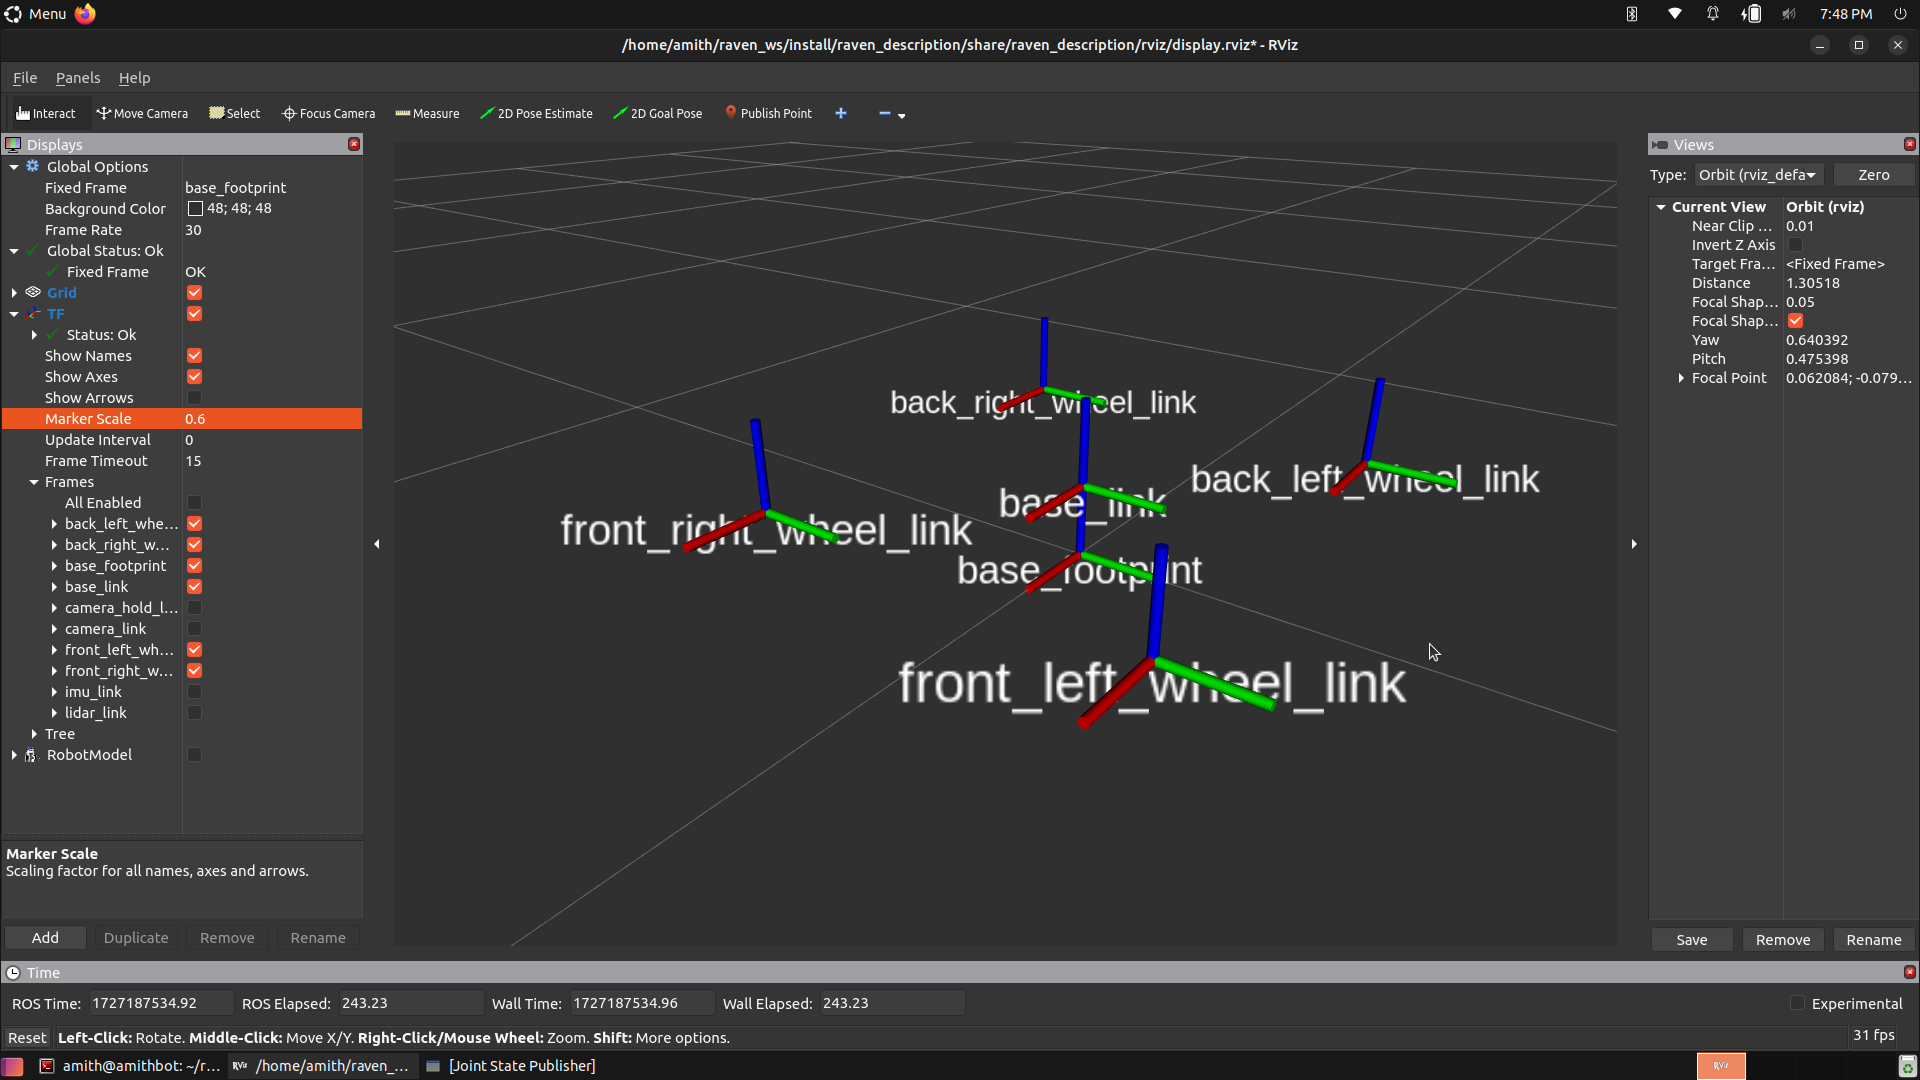
\includegraphics[scale=0.15]{images/Content/Transforms_Links}
			\caption{Transform links of the URDF}
			\label{fig:transformslinks}
		\end{figure}
		
		\begin{figure}[H]
			\centering
			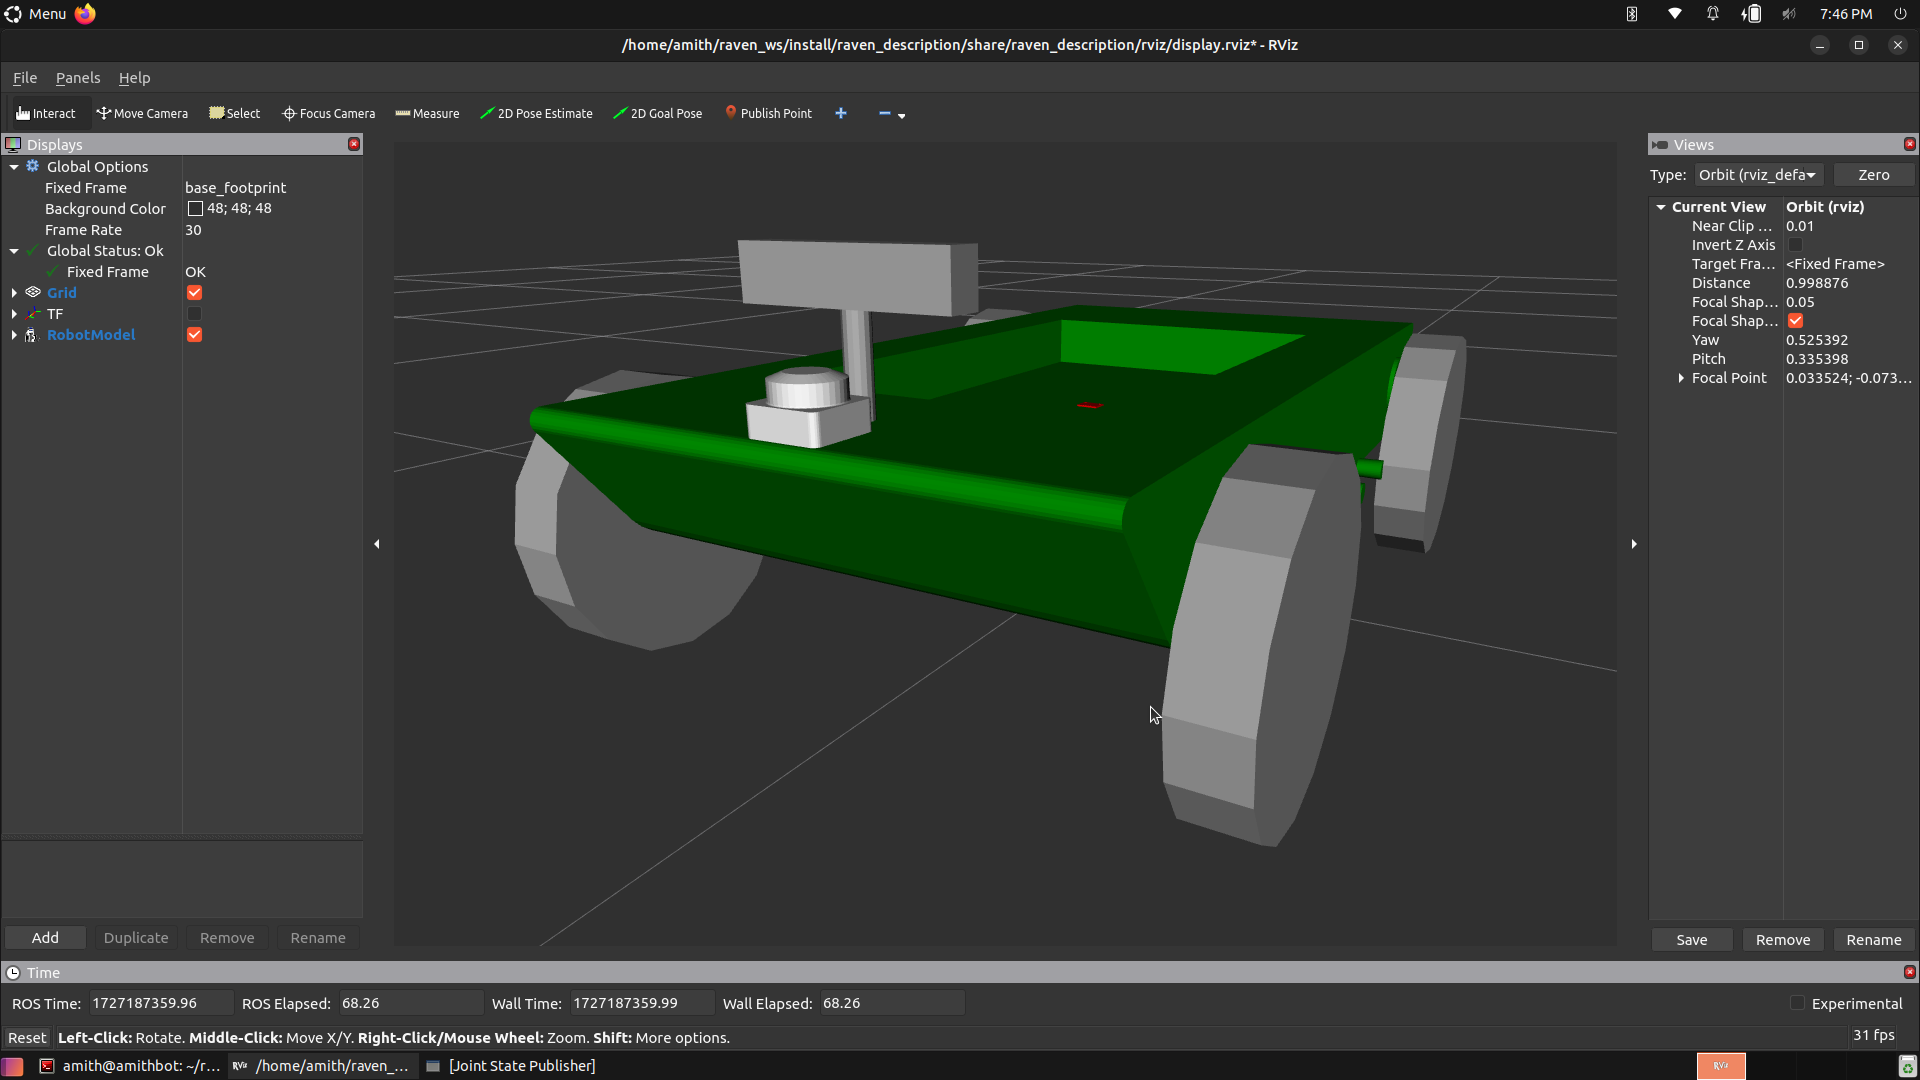
\includegraphics[scale=0.15]{images/Content/Basic_URDF_Model}
			\caption{Robot model of the URDF}
			\label{fig:basicurdfmodel}
		\end{figure}
		
		\begin{figure}[H]
			\centering
			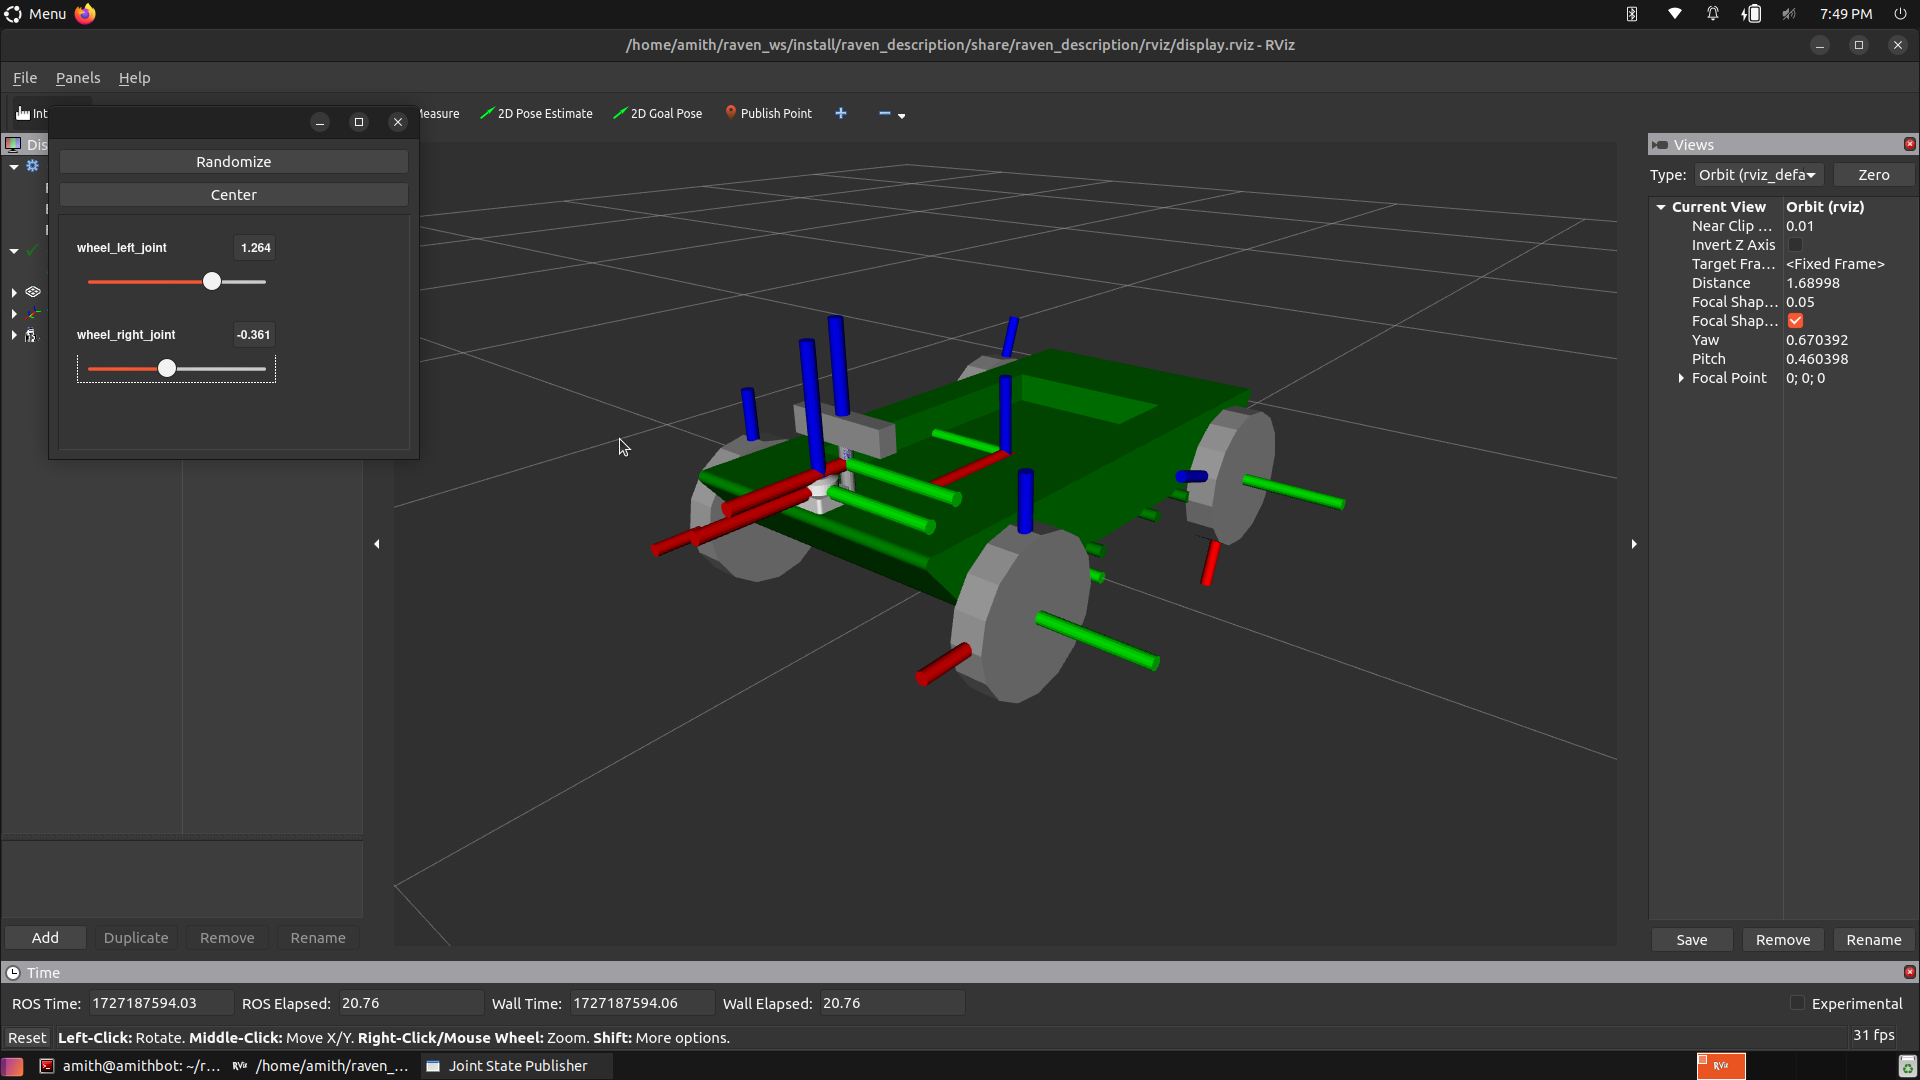
\includegraphics[scale=0.2]{images/Content/Rotation_of_wheels_using_JSP}
			\caption{Joint State Publisher GUI}
			\label{fig:wheelsusingjsp}
		\end{figure}
						
		
		\item \textbf{Robot visualization launch file created:} This is a configuration file used to start a
		visualization environment, allowing users to see the robot model in a graphical interface,
		typically using tools like Rviz.
		
		\item \textbf{GAZEBO simulation launch file created:} A launch file for Gazebo, a robotics simulator
		that enables the testing of robotic algorithms in a 3D environment, providing realistic
		physics and sensor feedback.
		
		\item \textbf{Simple controller:} A basic control algorithm that manages the robot's movements,
		typically involving direct input-output relationships without complex decision-making
		processes.
		
		\begin{figure}[H]
			\centering
			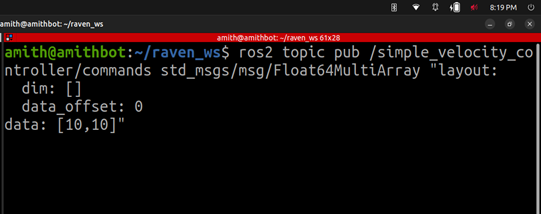
\includegraphics[scale=0.8]{images/Content/SImple_controller_drive}
			\caption{Simple controller command}
			\label{fig:simplecontrollerdrive}
		\end{figure}
		
		
		\item \textbf{Differential drive controller:} A control system specifically designed for robots with a
		differential drive mechanism, allowing them to navigate by varying the speed of each wheel
		independently.
		
		\begin{figure}[H]
			\centering
			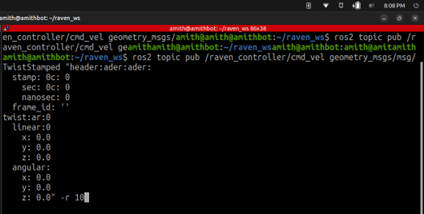
\includegraphics[scale=1.2]{images/Content/Differential_controller_drive}
			\caption{Differential drive controller command}
			\label{fig:differentialcontrollerdrive}
		\end{figure}
		
		
		\item \textbf{Noisy controller:} A controller designed to handle and compensate for noise in sensor data
		or actuator performance, ensuring more stable and reliable robot behavior during operation.
		
		\item \textbf{Kalman Filter:} An algorithm used for estimating the state of a dynamic system from a
		series of incomplete and noisy measurements, commonly used for sensor fusion in robotics.
		
		\begin{figure}[H]
			\centering
			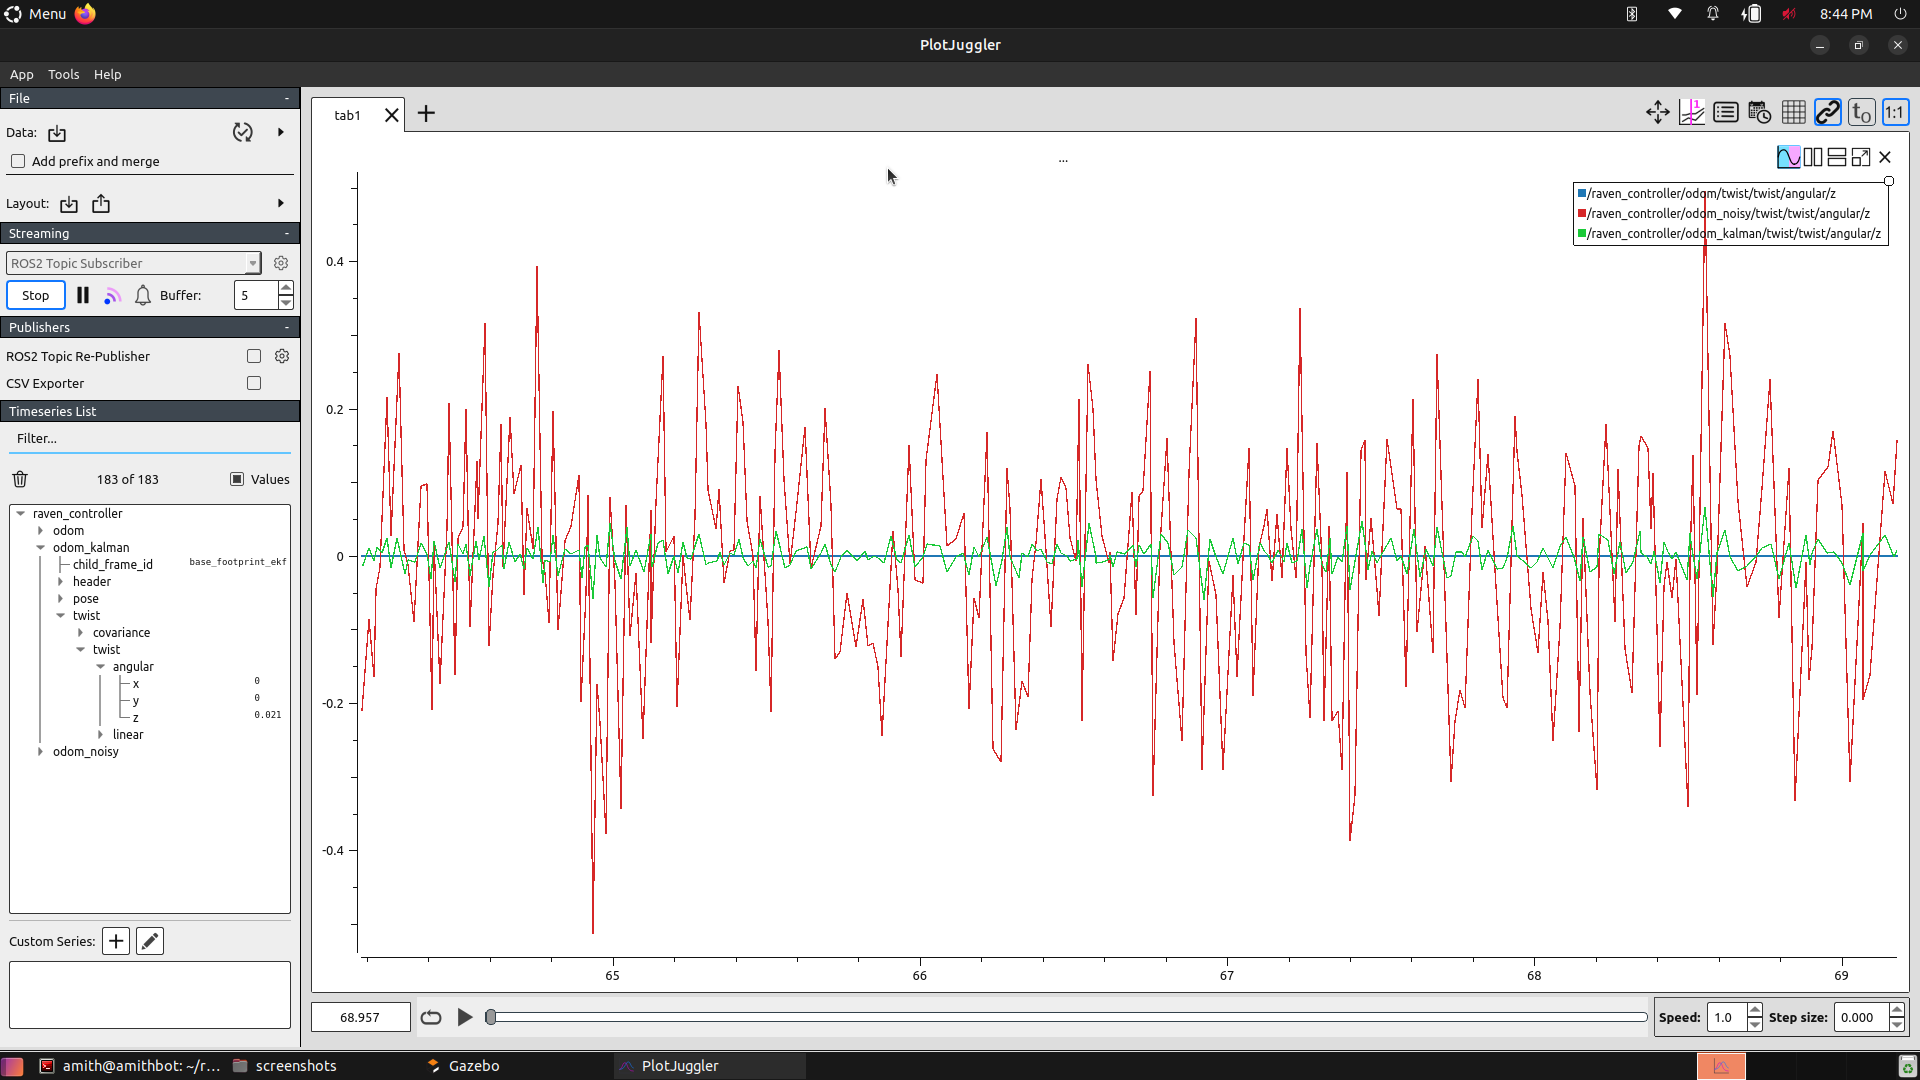
\includegraphics[scale=0.15]{images/Content/KALMAN_MOTION_FILTER}
			\caption{Kalman filtering the odometry values}
			\label{fig:kalmanmotionfilter}
		\end{figure}
		
		
		\item \textbf{Sensor integration:} The process of combining data from various sensors (e.g., LiDAR,
		cameras) to provide a comprehensive understanding of the robot's environment and
		enhance its decision-making capabilities.
		
		\begin{figure}[H]
			\centering
			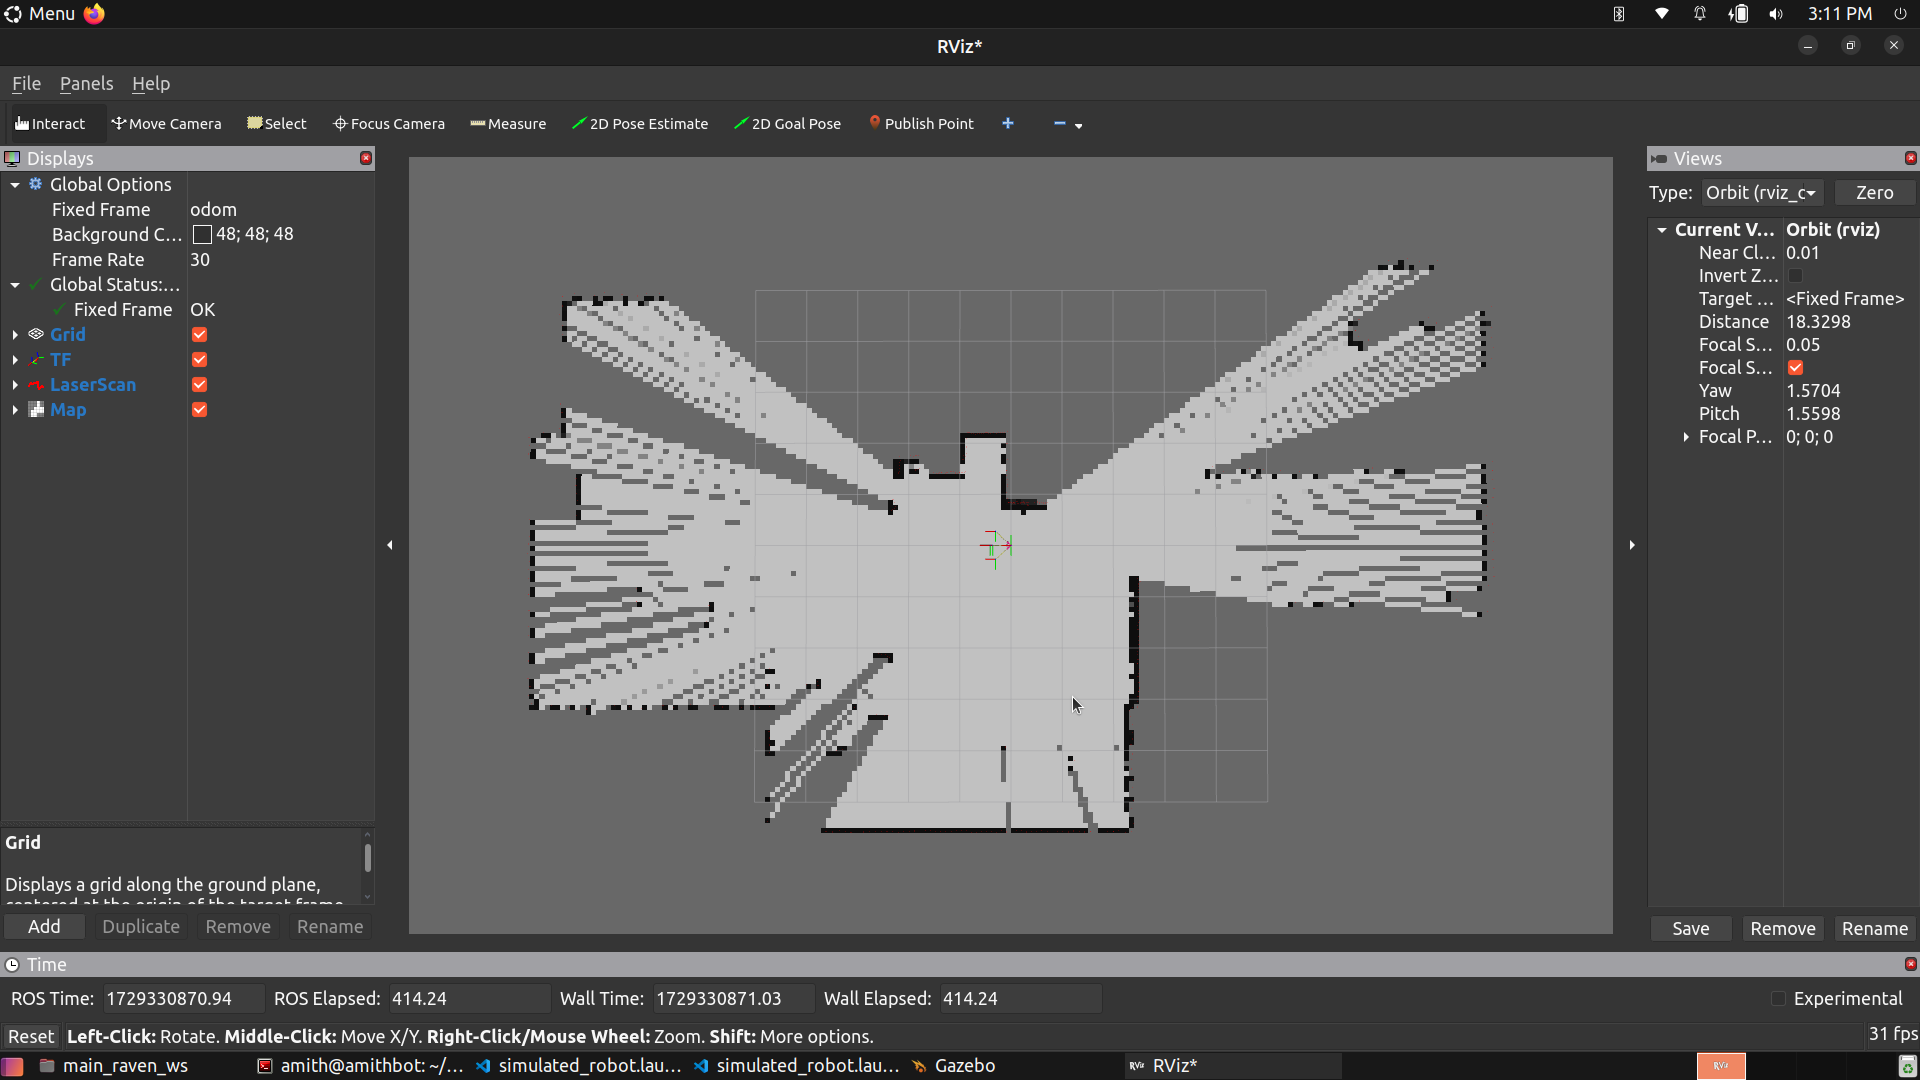
\includegraphics[scale=0.21]{images/Content/lidar_mapping}
			\caption{LiDAR mapping}
			\label{fig:lidarmapping}
		\end{figure}
		
		
		\item \textbf{Joystick Teleoperation:} A method for controlling the robot remotely using a joystick.
		Enables manual control of the robot's movements and actions.
		
		\begin{figure}[H]
			\centering
			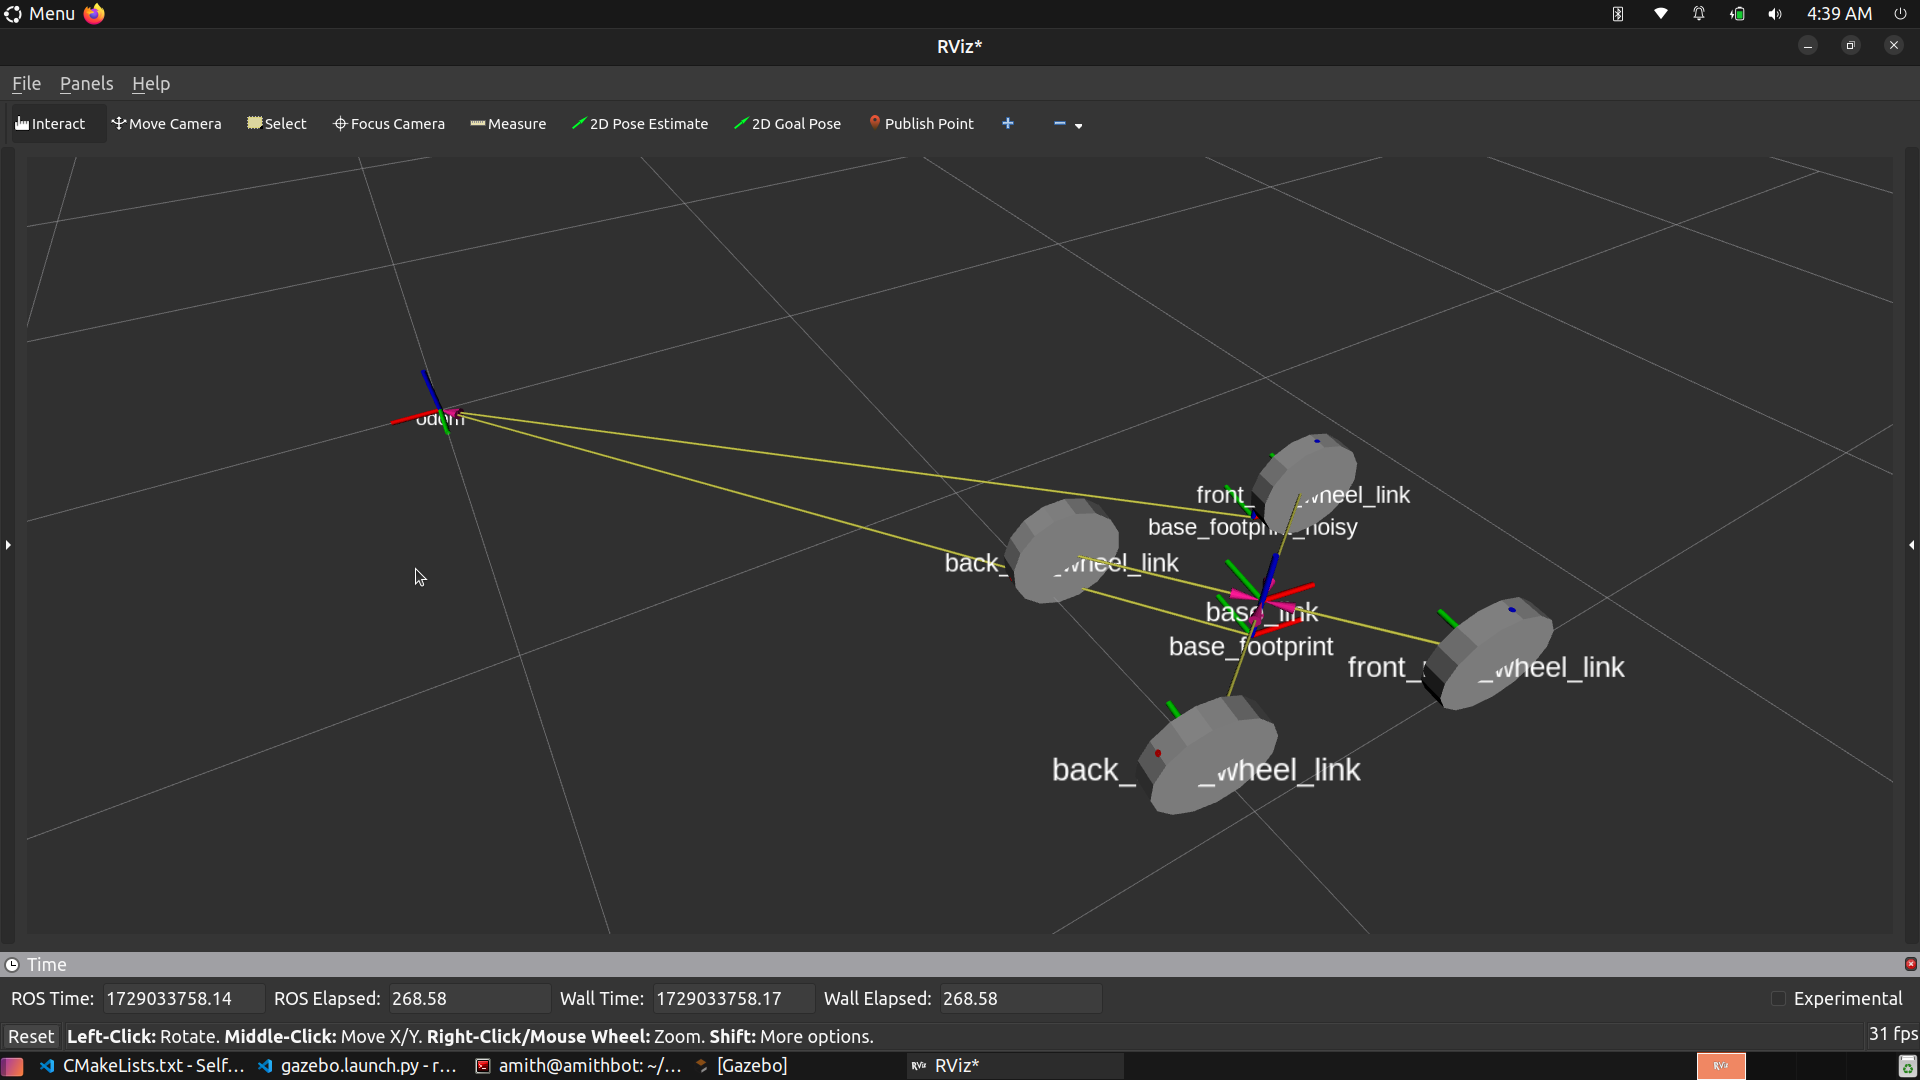
\includegraphics[scale=0.21]{images/Content/joystick_movement}
			\caption{Joystick teleoperation}
			\label{fig:joystickmovement}
		\end{figure}
		
		
		\item \textbf{NAV2 based simulation:} Utilizing the Navigation 2 framework for simulating robot
		navigation tasks, including path planning, obstacle avoidance, and goal reaching, typically
		in a simulated environment.
		
		\captionsetup[subfloat]{font={normalsize}}
		\begin{figure}[H]
			\centering
			\subfloat[Linear pose estimation]{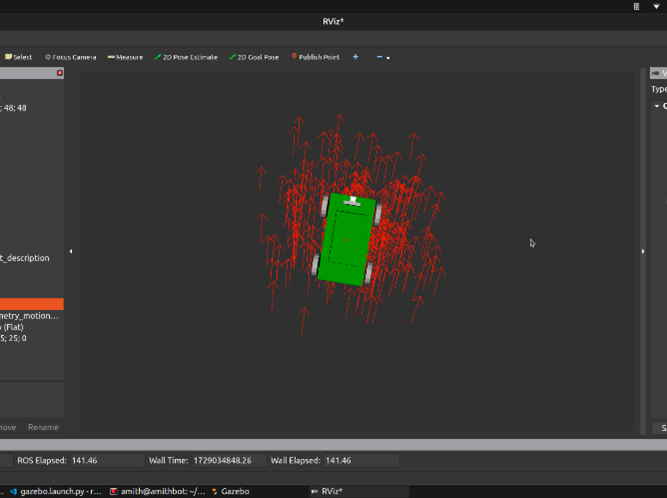
\includegraphics[width=0.45\textwidth]{images/Content/pose_estimation_linear movement.png}}
			\hfill
			\subfloat[Angular pose estimation]{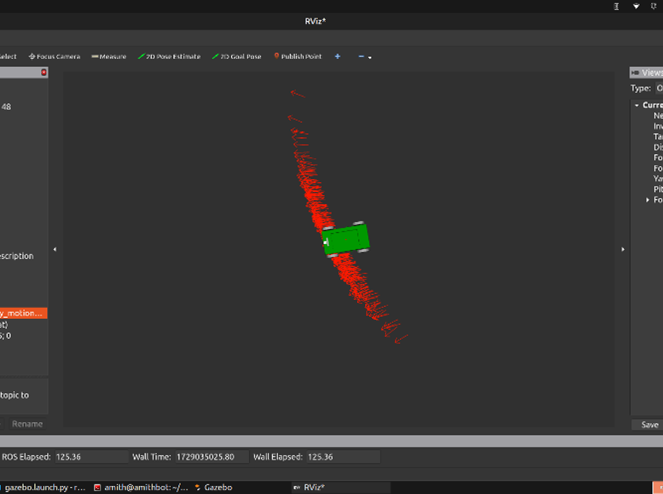
\includegraphics[width=0.45\textwidth]{images/Content/pose_noise_estimation_rotational.png}}
			\hfill
			\caption{Pose estimation}
			\label{fig:posestim}
		\end{figure}
		
		\begin{figure}[H]
			\centering
			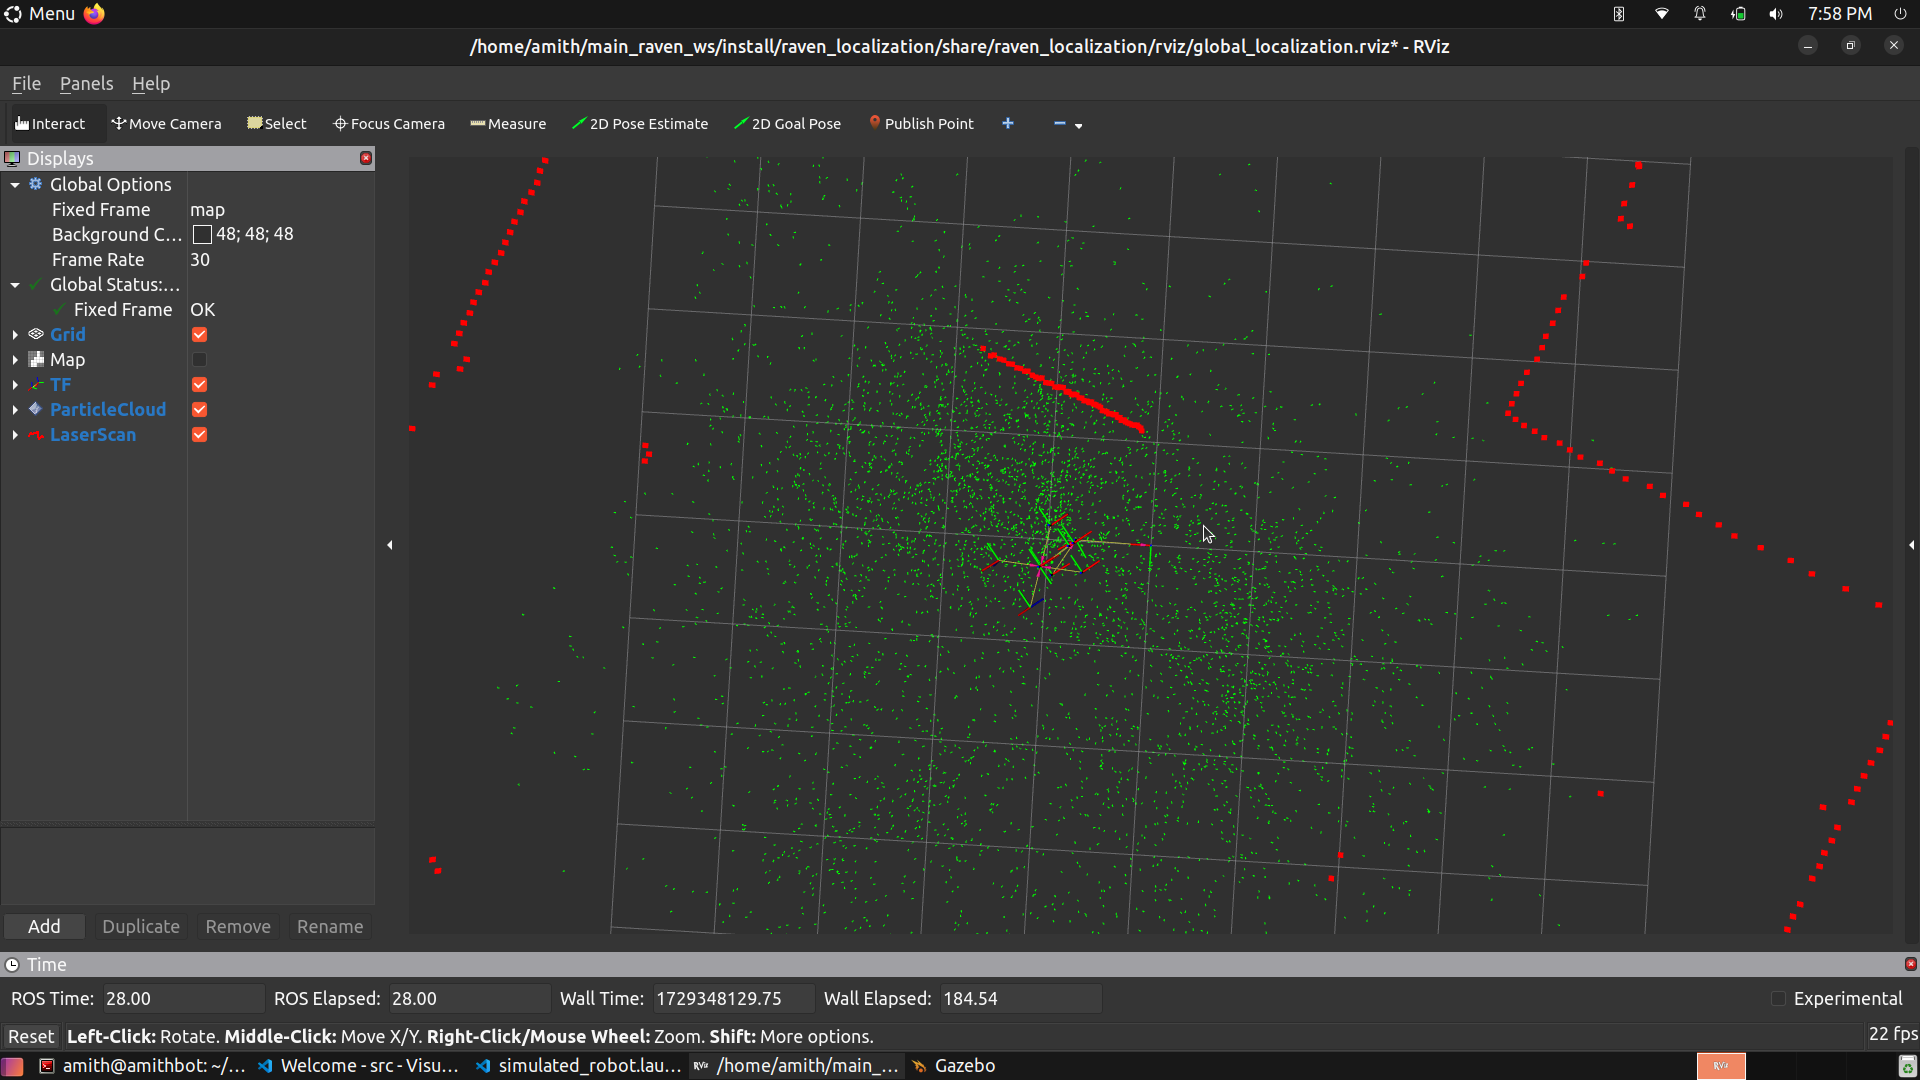
\includegraphics[scale=0.2]{images/Content/Nav2_AMCL.png}
			\caption{Nav2 AMCL}
			\label{fig:nav2amcl}
		\end{figure}
		
		\vspace{2in}
        
		\item \textbf{SLAM simulation:} SLAM (Simultaneous Localization and Mapping) involves creating a
		map of an unknown environment while simultaneously keeping track of the robot's location
		within that environment, typically simulated in a controlled setting.
		
		\captionsetup[subfloat]{font={normalsize}}
		\begin{figure}[H]
			\centering
			\subfloat[Low accuracy SLAM]{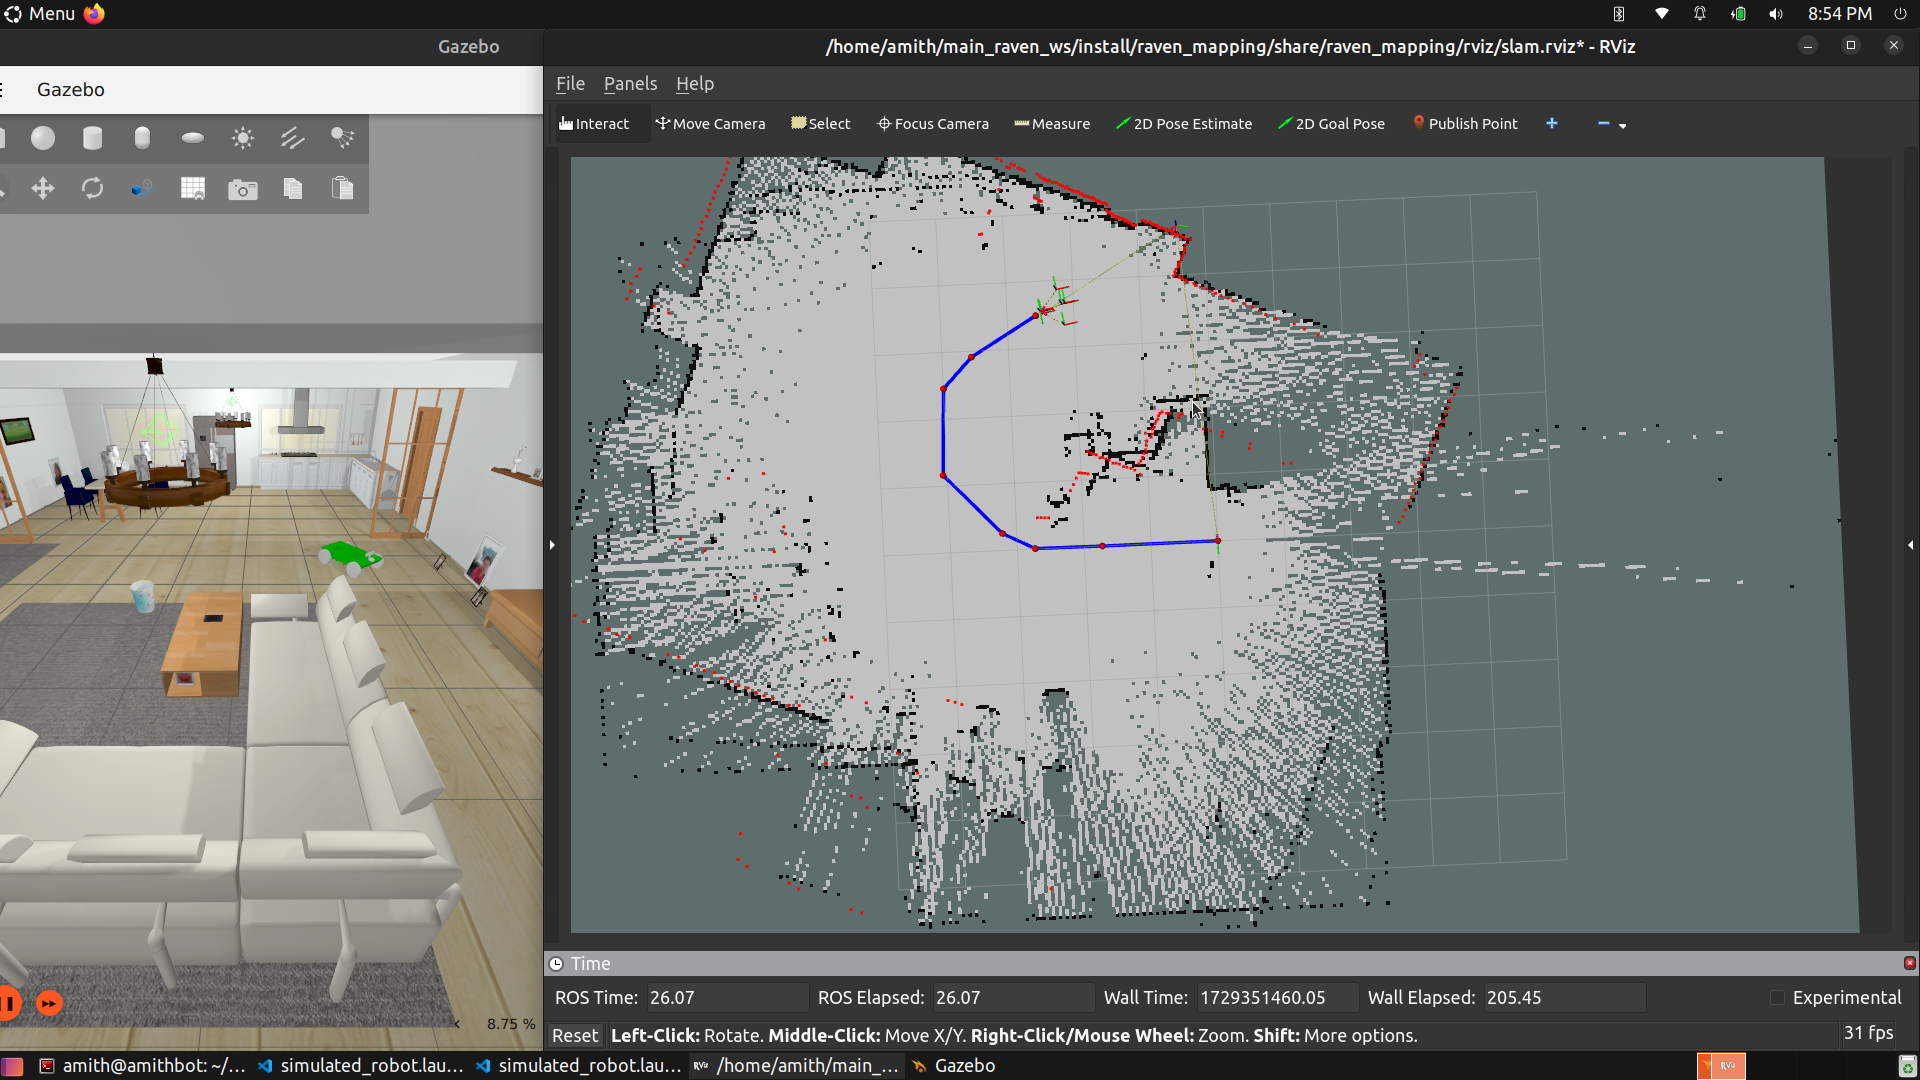
\includegraphics[width=0.45\textwidth]{images/Content/SLAM_2.png}}
			\hfill
			\subfloat[High accuracy SLAM]{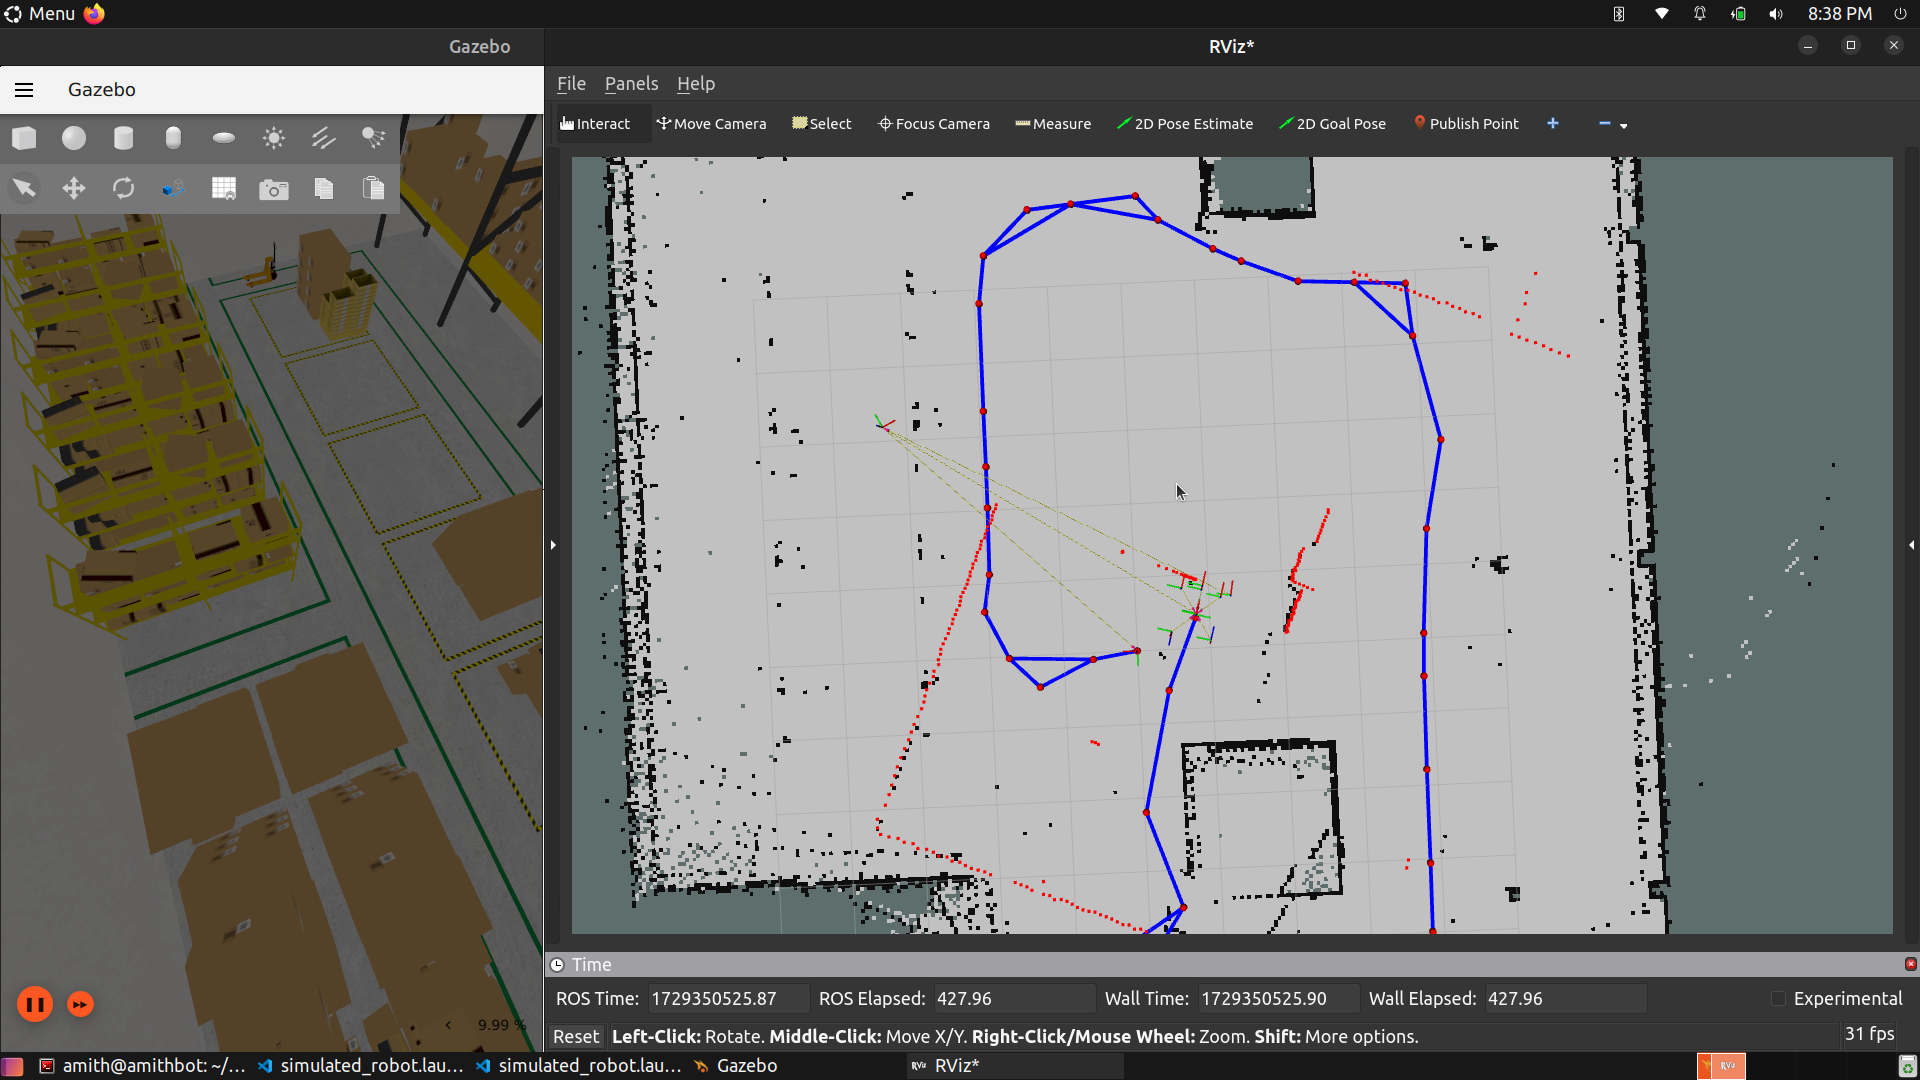
\includegraphics[width=0.45\textwidth]{images/Content/SLAM.png}}
			\hfill
			\caption{SLAM}
			\label{fig:slamsim}
		\end{figure}
		
		\item \textbf{Final Robot firmware launch file created:} A launch file that initializes and executes the
		final firmware code on the robot, encompassing all necessary configurations and
		parameters for the robot to operate effectively in real-world scenarios. These components
		collectively contribute to the overall functionality and performance of the robotic system
		under development. \emph{“simulated\_robot.launch.py”}.
		
		\item \textbf{IMU Simulation in WOKWI:} A simulation environment for testing and validating IMU (Inertial Measurement Unit) functionality using WOKWI. This setup allows for real-time testing of IMU data processing and integration before hardware deployment.
		
		\begin{figure}[H]
			\centering
			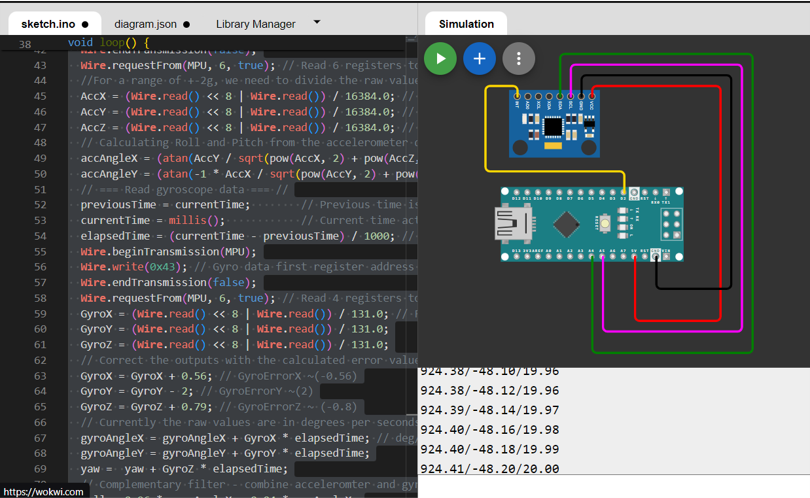
\includegraphics[scale=0.35]{images/Content/Imu_sim_wokwi}
			\caption{IMU Simulation in WOKWI}
		\end{figure}
		
		\item \textbf{IMU Interfacing with Arduino Nano:} A demonstration of IMU integration with an Arduino Nano microcontroller. This setup enables the collection and processing of IMU data for motion tracking and orientation estimation in small-scale robotics applications.
		
		\begin{figure}[H]
			\centering
			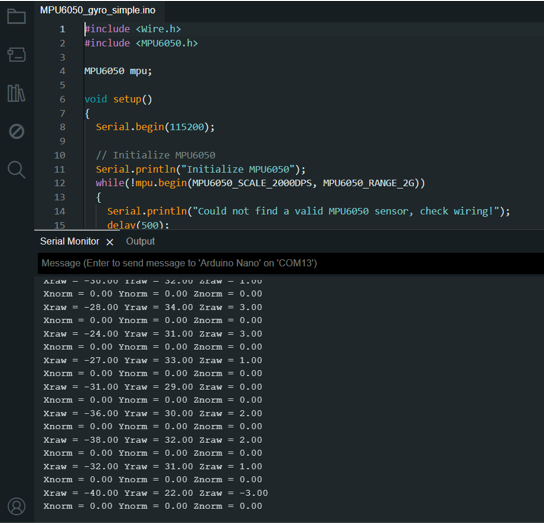
\includegraphics[scale=0.5]{images/Content/Imu_Inter_arduino_nano}
			\caption{IMU Interfacing with Arduino Nano}
		\end{figure}
		
		\item \textbf{IMU Interfacing with Jetson Orin Nano:} A high-performance IMU integration with the Jetson Orin Nano platform. This configuration supports advanced data processing and real-time analytics for robotics applications requiring high computational power.
		
		\begin{figure}[H]
			\centering
			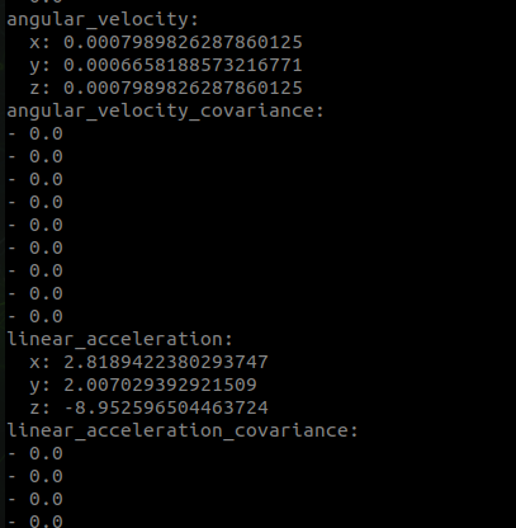
\includegraphics[scale=0.5]{images/Content/IMU_JETSON}
			\caption{IMU Interfacing with Jetson Orin Nano}
		\end{figure}
		
		\item \textbf{IMU Interfacing and Visualization:} A visualization of IMU data using RVIZ, a robotics visualization tool. This setup provides real-time feedback on IMU orientation and motion, aiding in system calibration and performance monitoring.
		
		\begin{figure}[H]
			\centering
			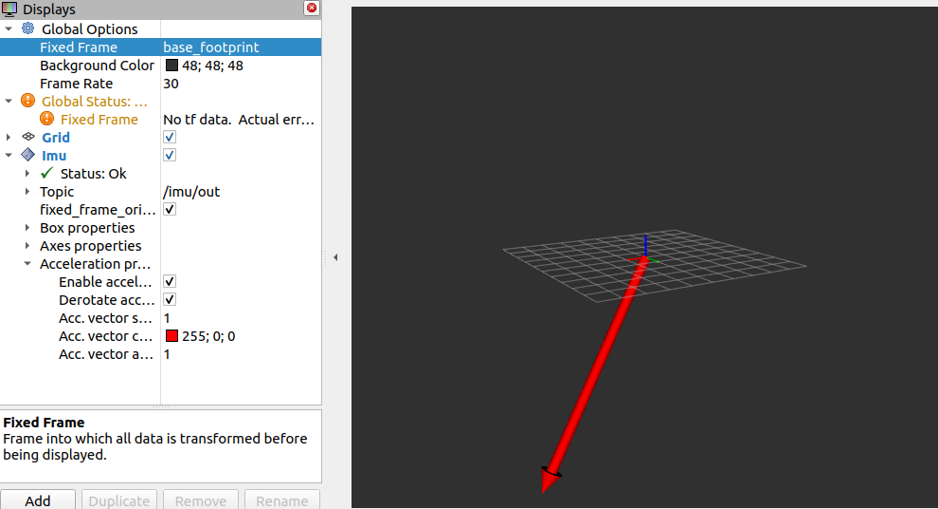
\includegraphics[scale=0.6]{images/Content/IMU_RVIZ}
			\caption{IMU Interfacing and Visualization}
		\end{figure}
		
		\item \textbf{IMU Structure Calibration:} A detailed process of calibrating the IMU holder to ensure accurate sensor alignment and leveling. Proper calibration is critical for precise motion tracking and orientation estimation in robotics applications.
		
		\captionsetup[subfloat]{font={normalsize}}
		\begin{figure}[H]
			\centering
			\subfloat[IMU holder]{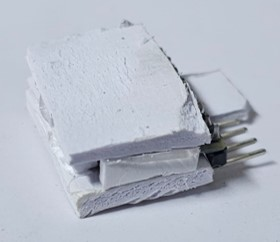
\includegraphics[width=0.45\textwidth]{images/Content/Imu_Holder}}
			\hfill
			\subfloat[IMU holder leveling]{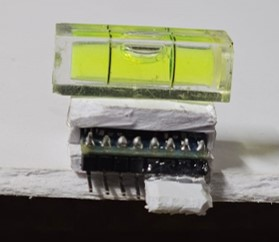
\includegraphics[width=0.45\textwidth]{images/Content/Imu_Holder_Calib}}
			\hfill
			\caption{IMU Structure Calibration}
		\end{figure}


        \item \textbf{Internal System Wiring:} Internal system wiring organizes electrical connections for reliable communication between components, enhancing reliability and simplifying troubleshooting. Clear documentation supports integration, maintenance, and performance monitoring.
		\captionsetup[subfloat]{font={normalsize}}
		\begin{figure}[H]
			\centering
			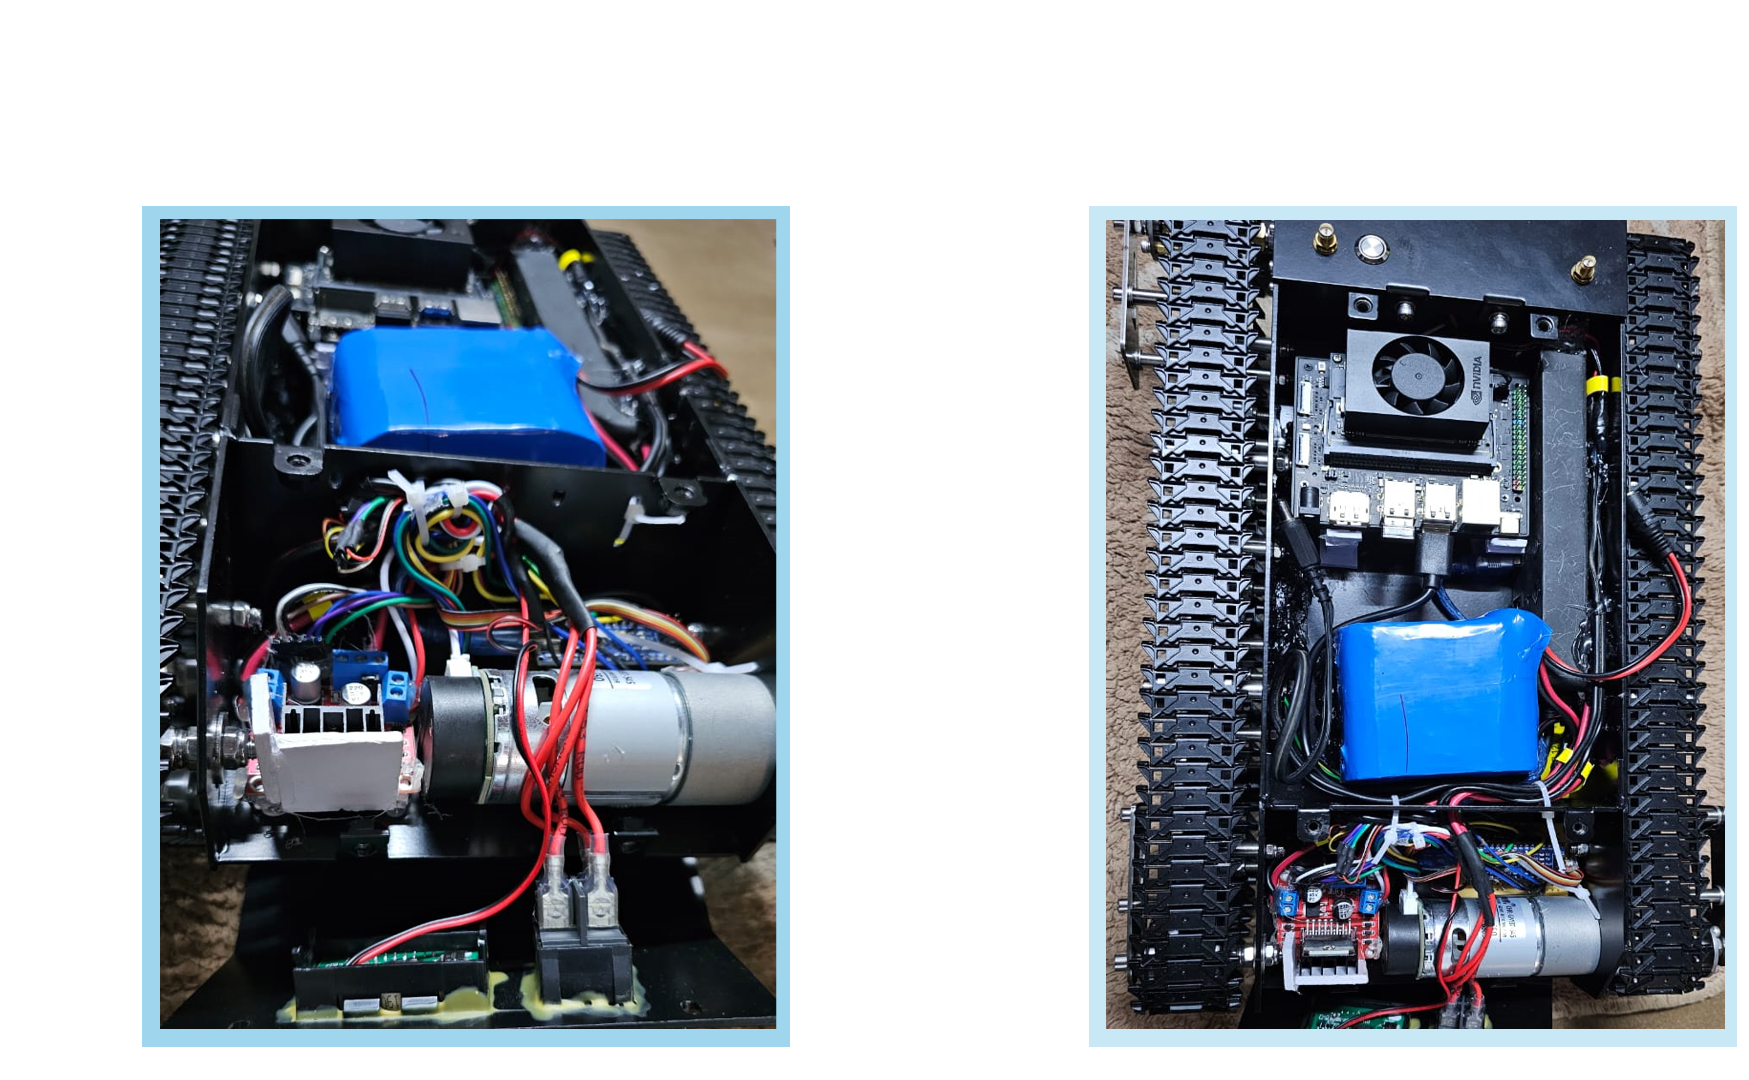
\includegraphics[scale=0.5]{images/Content/Internal_Wiring_1.png}
			\caption{Internal System Wiring}
		\end{figure}

        \item \textbf{RPLIDAR Placement:} Strategic RPLIDAR placement ensures optimal scanning, minimizes obstructions, and enhances mapping and navigation. Key considerations include height, angle, and stable mounting to maximize performance and ensure consistent data collection.
		
		\begin{figure}[H]
			\centering
			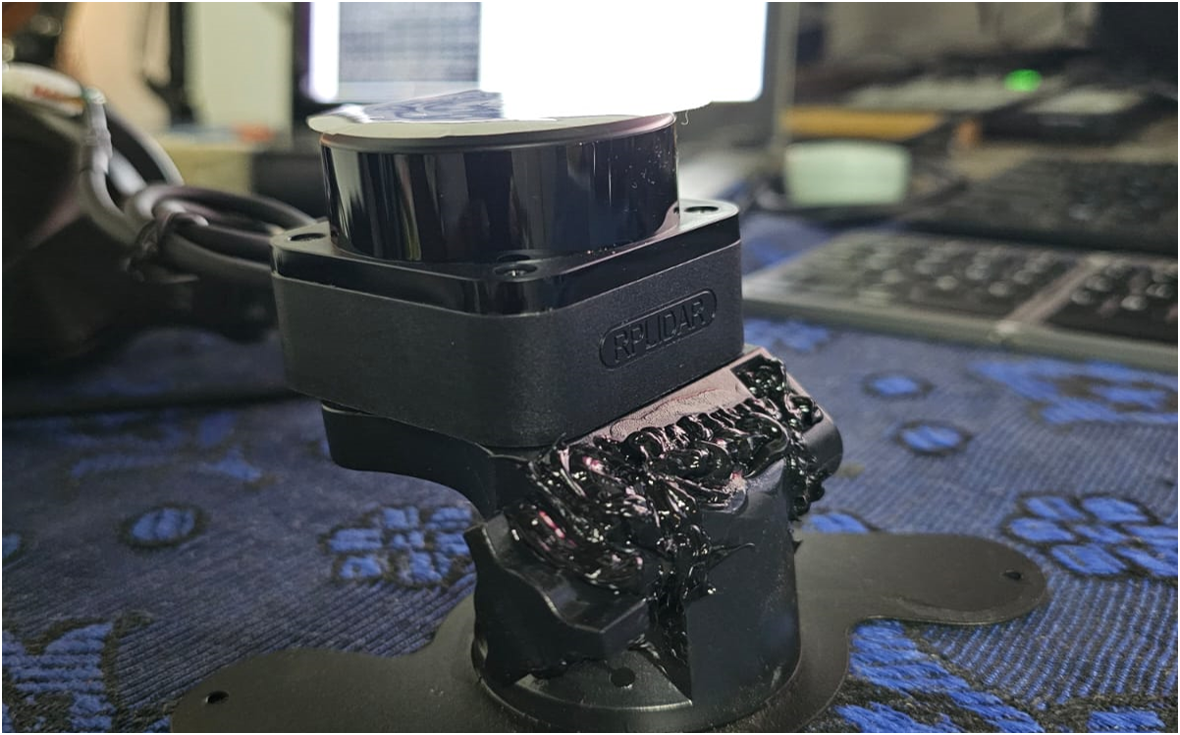
\includegraphics[scale=0.4]{images/Content/RPLIDAR_PLACEMENT.png}
			\caption{RPLIDAR Placement}
		\end{figure}
	\end{enumerate}
}
